% RQ2 Results: Governance Capture Mitigation

\subsection{Overview}

We present results from \experimentruns{} simulation runs across 27 mitigation configurations. Table~\ref{tab:rq2-overview} summarizes the experimental scope.

\begin{table}[htbp]
\centering
\caption{RQ2 Results Overview (Experiment 04)}
\label{tab:rq2-overview}
\begin{tabular}{lr}
\toprule
Parameter & Value \\
\midrule
Mitigation configurations & 27 \\
Runs per configuration & 25 \\
Total simulation runs & 675 \\
\bottomrule
\end{tabular}
\end{table}

\subsection{Vote Cap Effects}

\subsubsection{Whale Influence Reduction}

\begin{figure}[htbp]
    \centering
    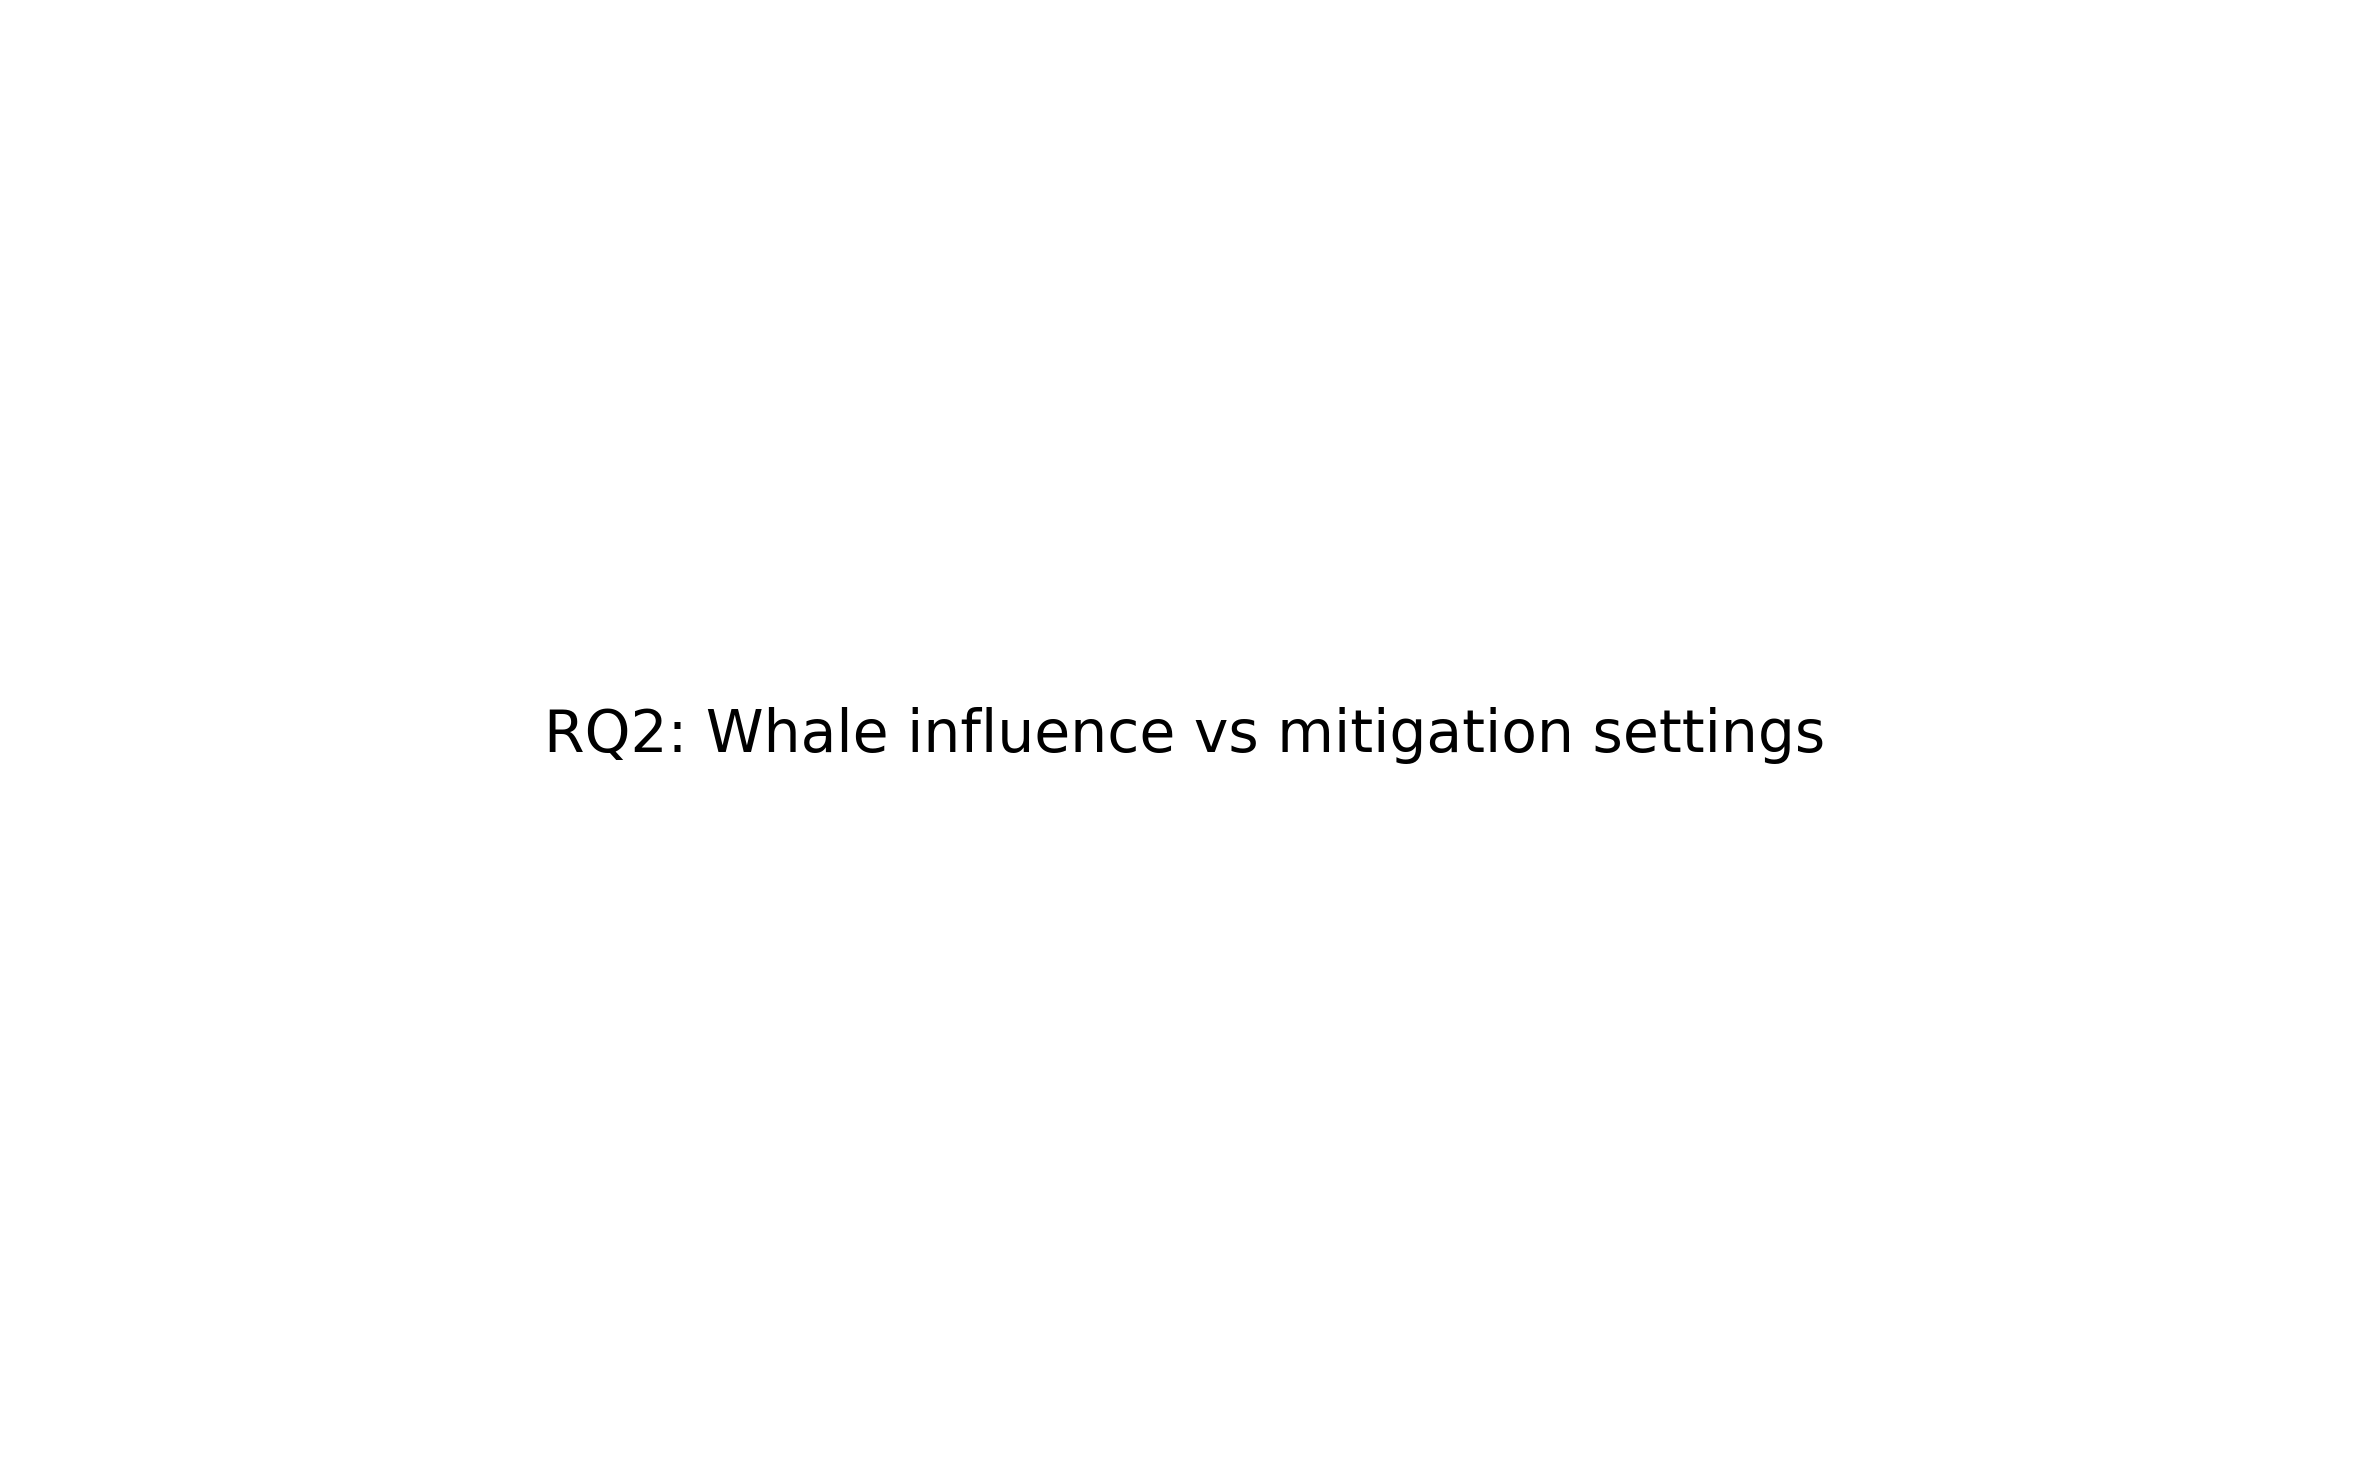
\includegraphics[width=0.8\textwidth]{../figures/rq2_whale_influence}
    \caption{Whale influence (top-10 share) under different vote cap settings. Caps effectively reduce peak influence, with 2\% cap achieving largest reduction. Error bars show 95\% CI.}
    \label{fig:rq2-whale-influence}
\end{figure}

\begin{table}[htbp]
\centering
\caption{Whale influence by vote cap setting}
\label{tab:rq2-caps}
\begin{tabular}{lccc}
\toprule
Cap Setting & Whale Influence & Nakamoto & Pass Rate \\
\midrule
\pl{None} & \pl{--} & \pl{--} & \pl{--} \\
\pl{5\%} & \pl{--} & \pl{--} & \pl{--} \\
\pl{2\%} & \pl{--} & \pl{--} & \pl{--} \\
\bottomrule
\end{tabular}
\end{table}

\subsection{Quadratic Voting Effects}

\subsubsection{Power Distribution Compression}

\begin{figure}[htbp]
    \centering
    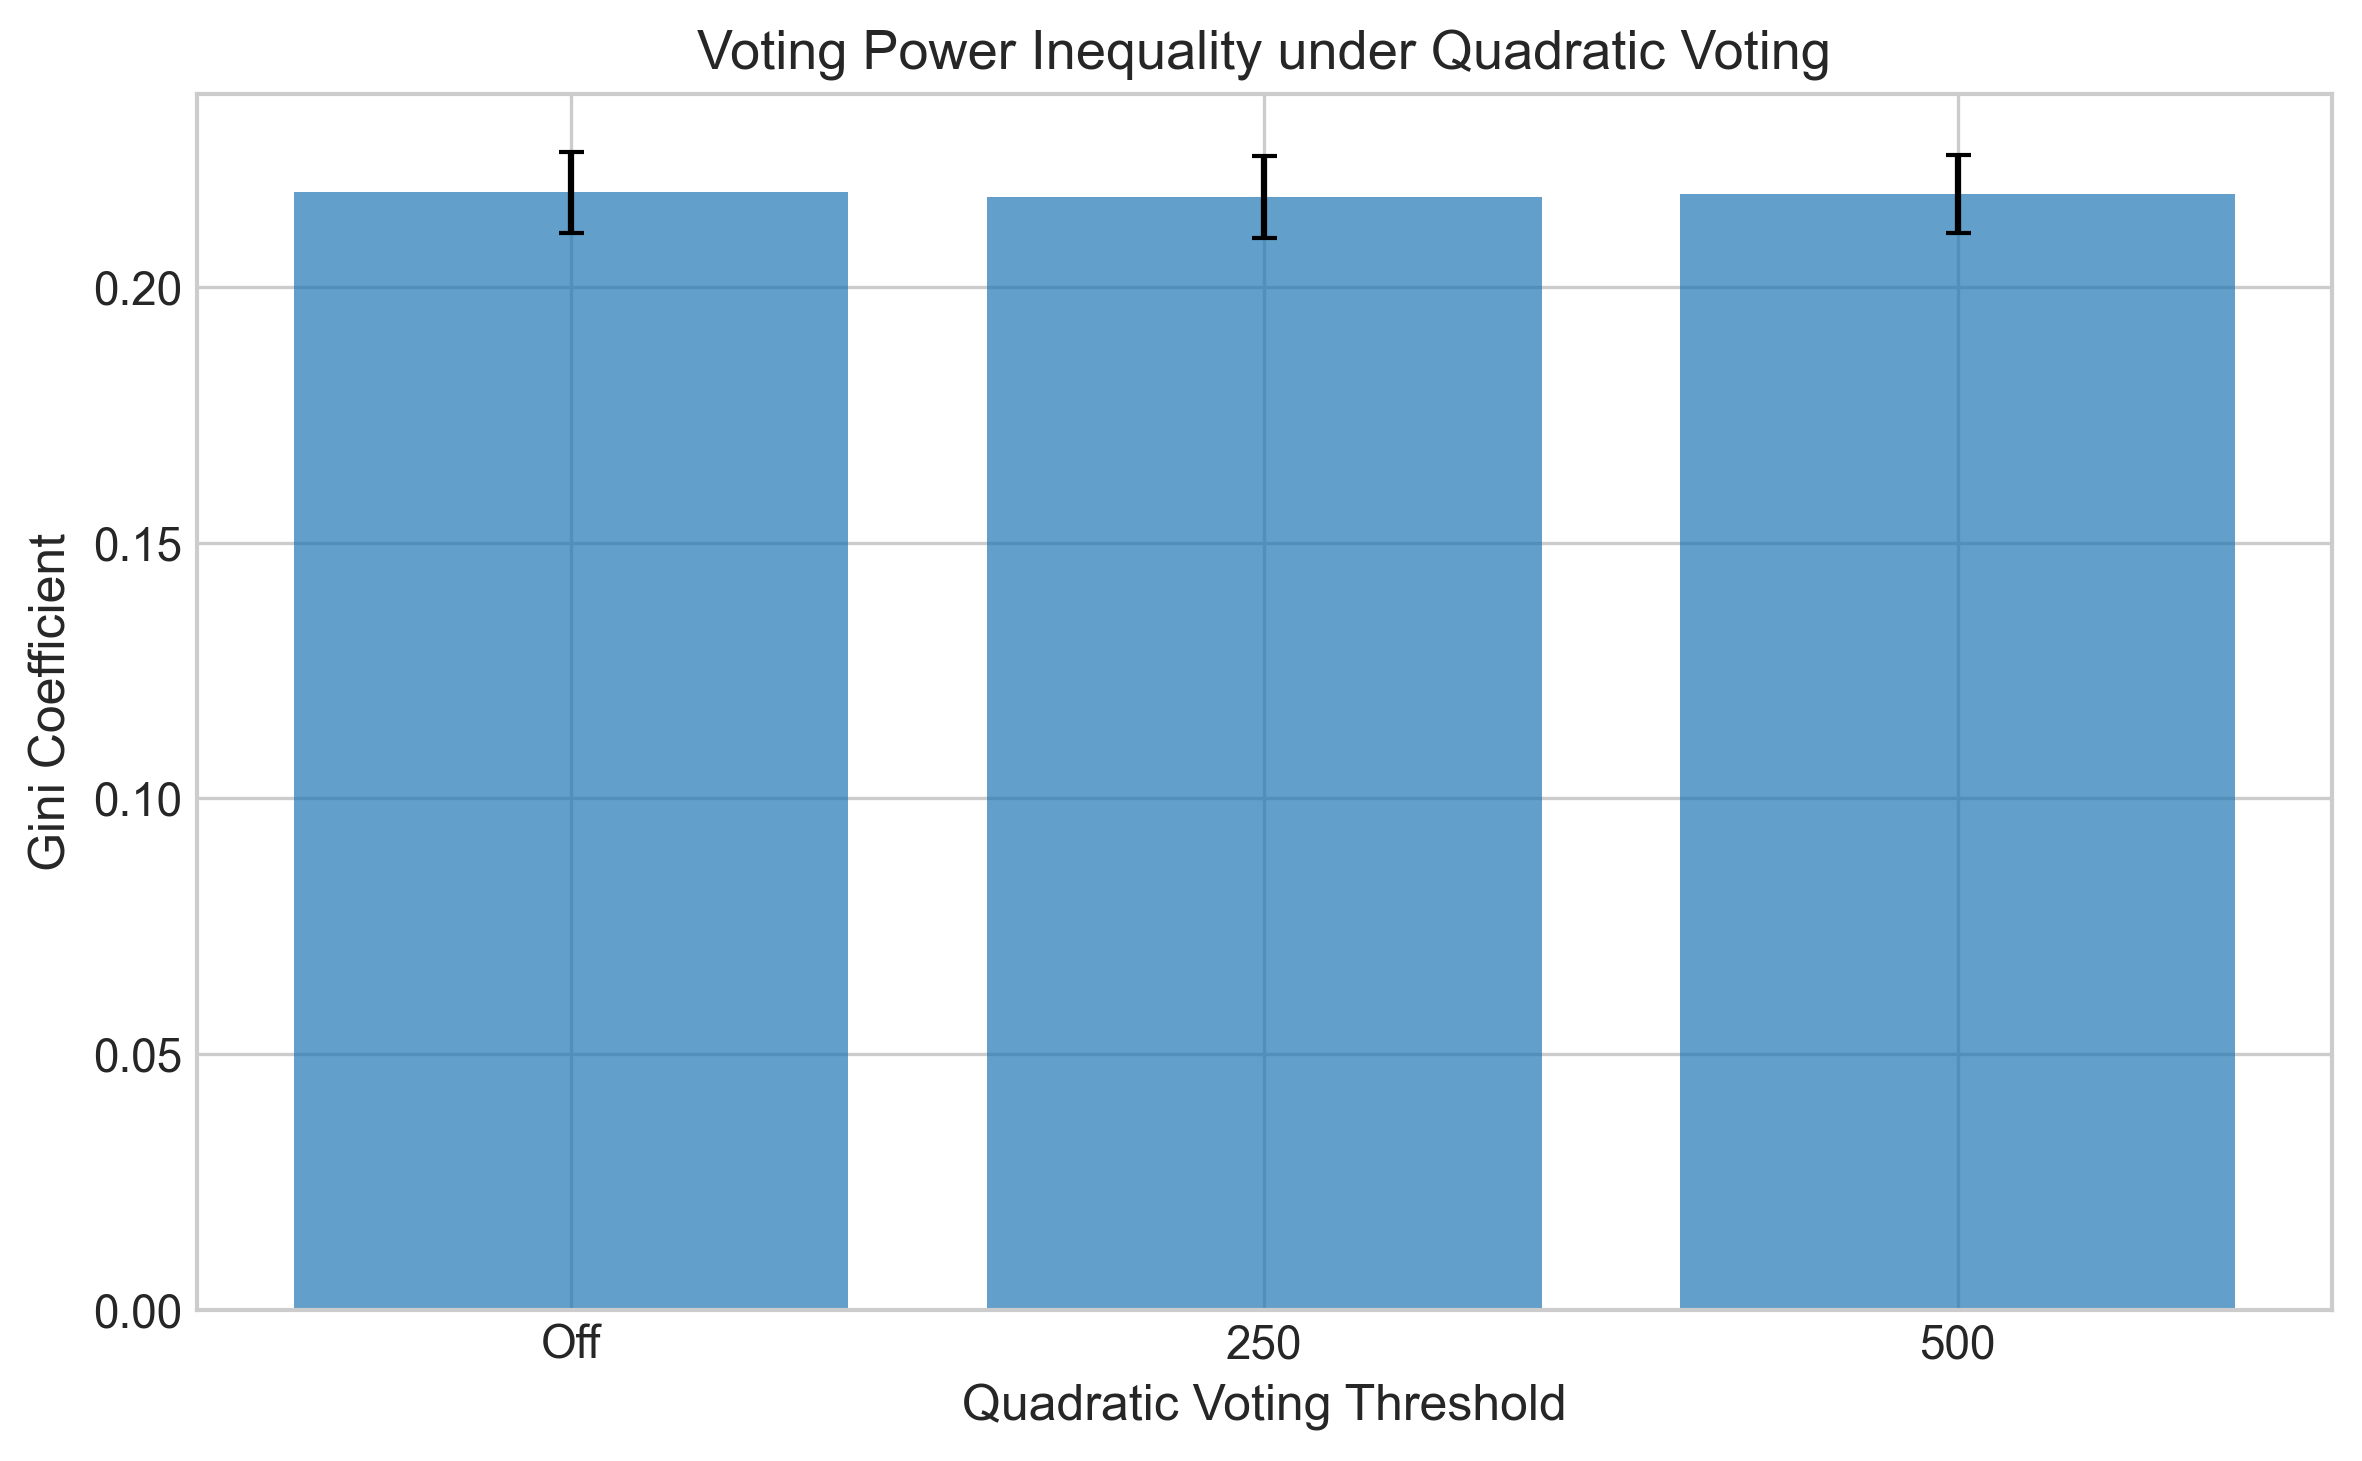
\includegraphics[width=0.8\textwidth]{../figures/rq2_gini_quad}
    \caption{Voting power Gini coefficient under linear, square root, and cube root scaling. Quadratic mechanisms compress inequality substantially.}
    \label{fig:rq2-gini-quad}
\end{figure}

\begin{table}[htbp]
\centering
\caption{Power distribution by quadratic setting}
\label{tab:rq2-quad}
\begin{tabular}{lccc}
\toprule
Scaling & Gini (Voting Power) & Whale Influence & Nakamoto \\
\midrule
\pl{Linear} & \pl{--} & \pl{--} & \pl{--} \\
\pl{Square root} & \pl{--} & \pl{--} & \pl{--} \\
\pl{Cube root} & \pl{--} & \pl{--} & \pl{--} \\
\bottomrule
\end{tabular}
\end{table}

\subsection{Velocity Penalty Effects}

\subsubsection{Attack Prevention}

\begin{figure}[htbp]
    \centering
    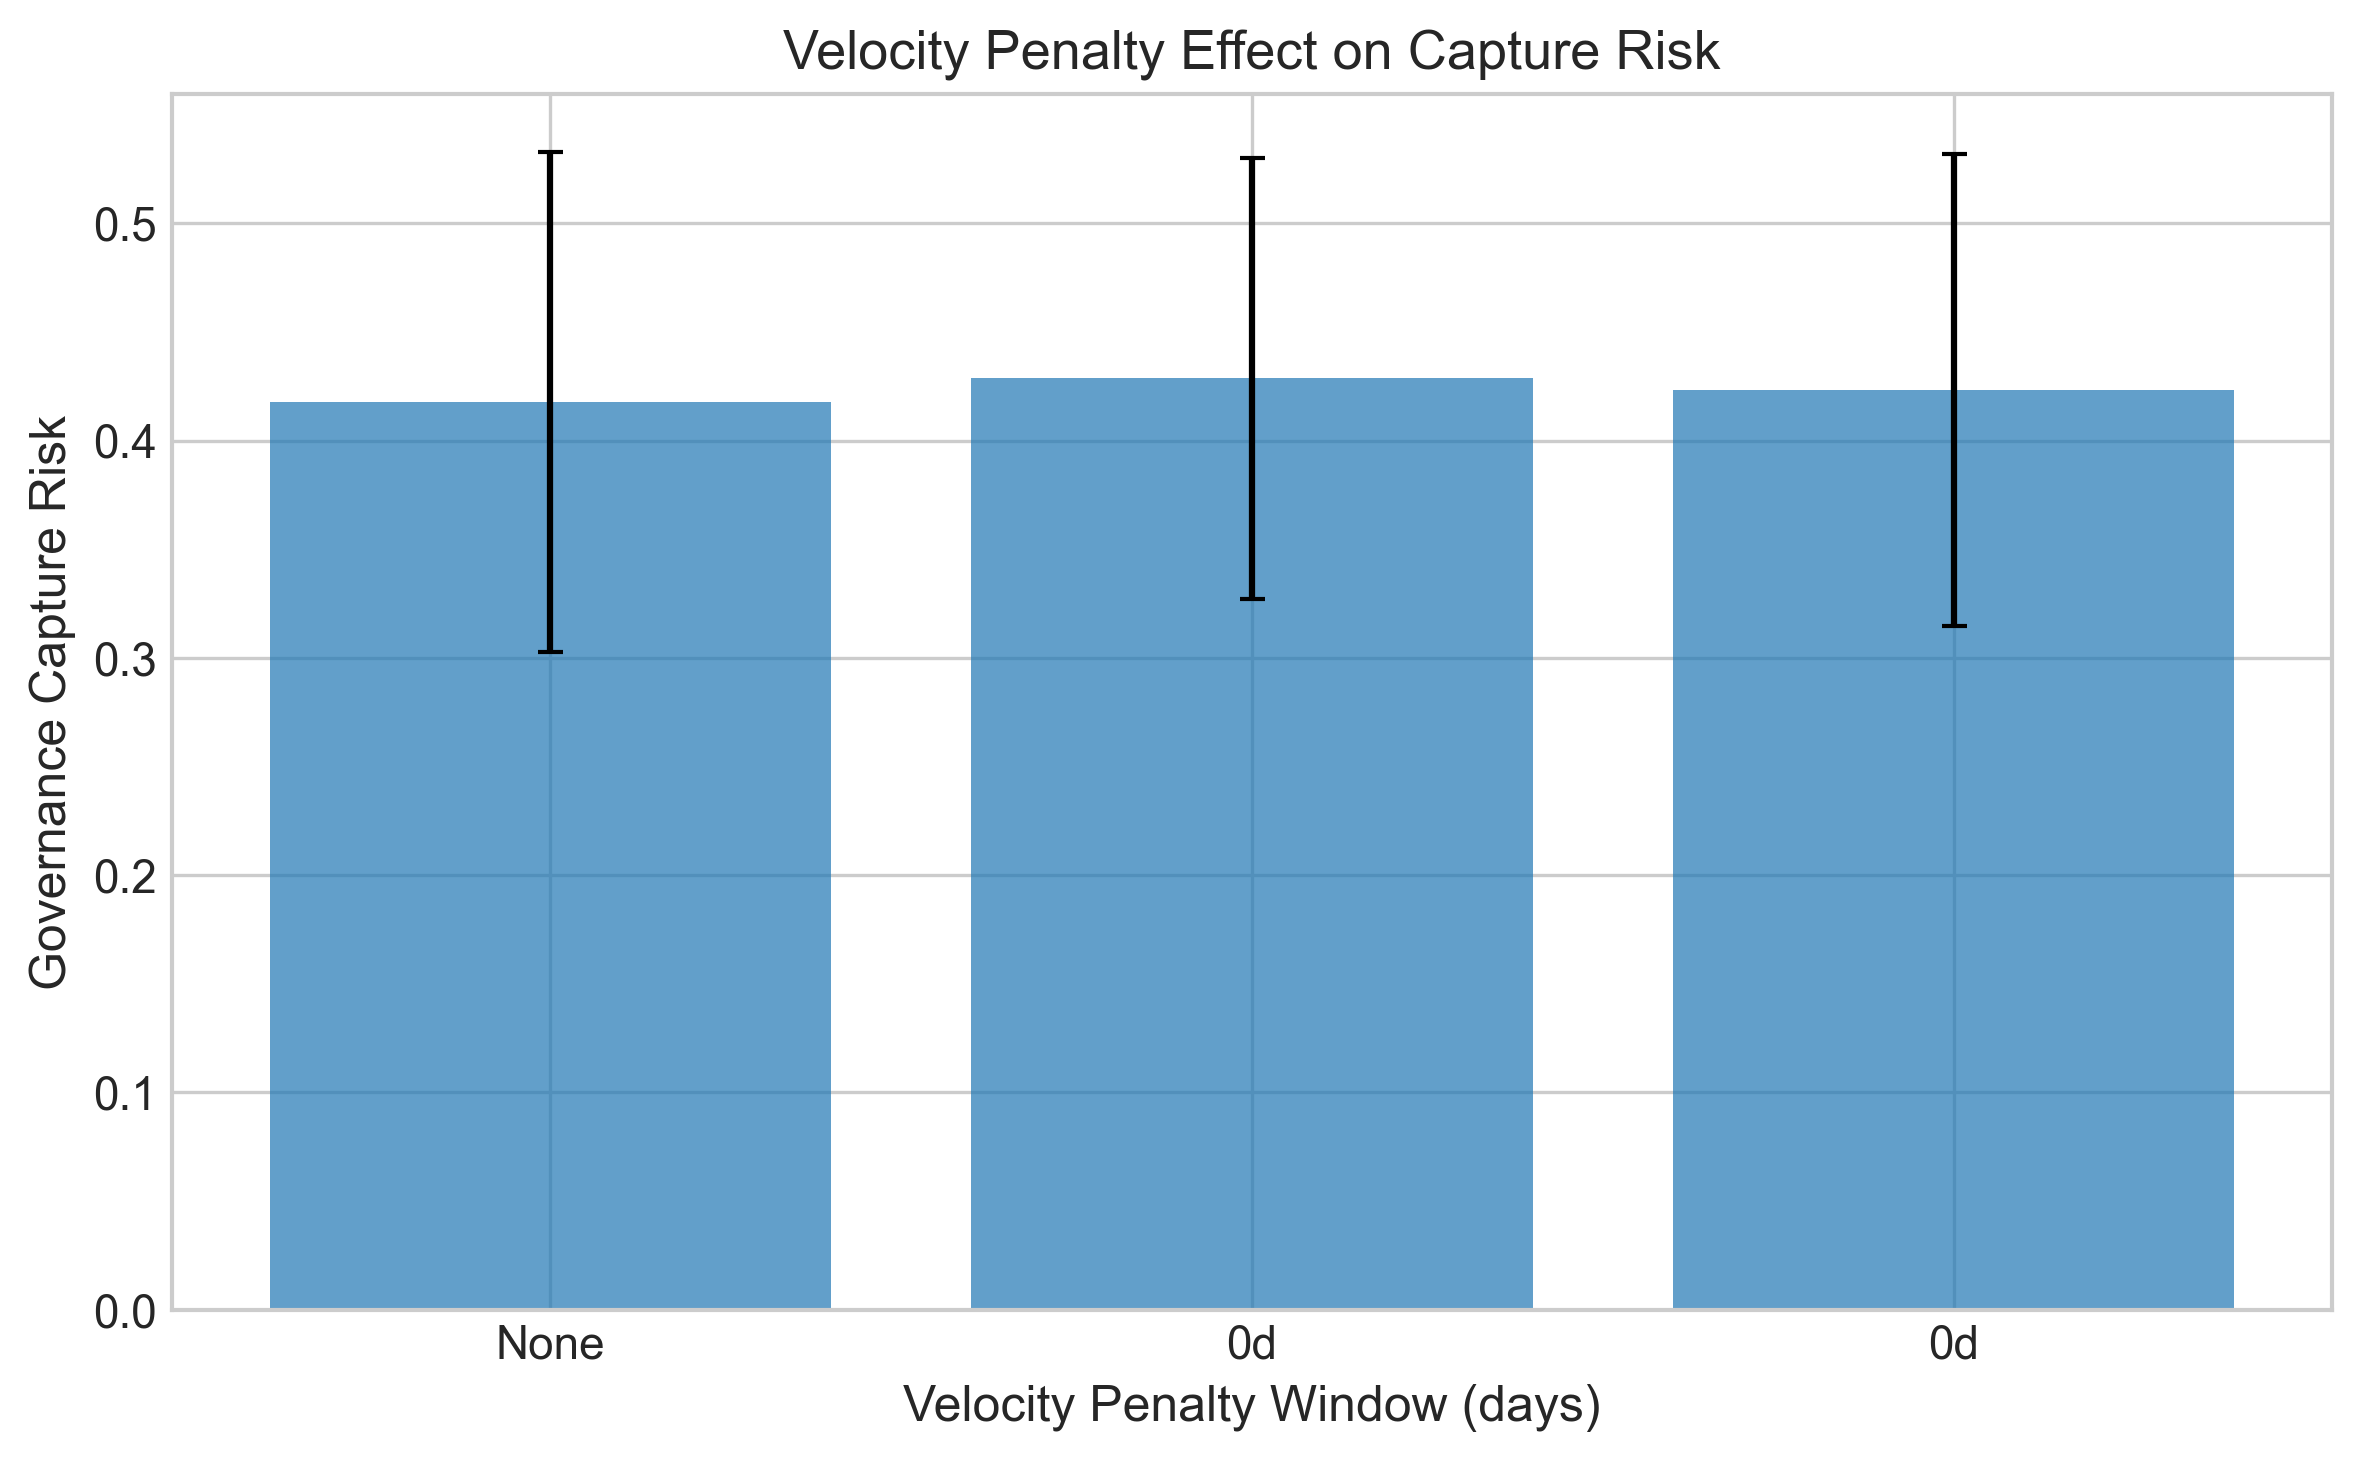
\includegraphics[width=0.8\textwidth]{../figures/rq2_velocity}
    \caption{Effectiveness of velocity penalties against simulated accumulation attacks. Longer windows provide stronger protection but may disadvantage new participants.}
    \label{fig:rq2-velocity}
\end{figure}

\begin{table}[htbp]
\centering
\caption{Velocity penalty effects}
\label{tab:rq2-velocity}
\begin{tabular}{lccc}
\toprule
Window & Attack Success Rate & New Participant Impact & Pass Rate \\
\midrule
\pl{None} & \pl{--} & \pl{--} & \pl{--} \\
\pl{30-day} & \pl{--} & \pl{--} & \pl{--} \\
\pl{90-day} & \pl{--} & \pl{--} & \pl{--} \\
\bottomrule
\end{tabular}
\end{table}

\subsection{Combined Mechanisms}

\subsubsection{Interaction Effects}

\begin{figure}[htbp]
    \centering
    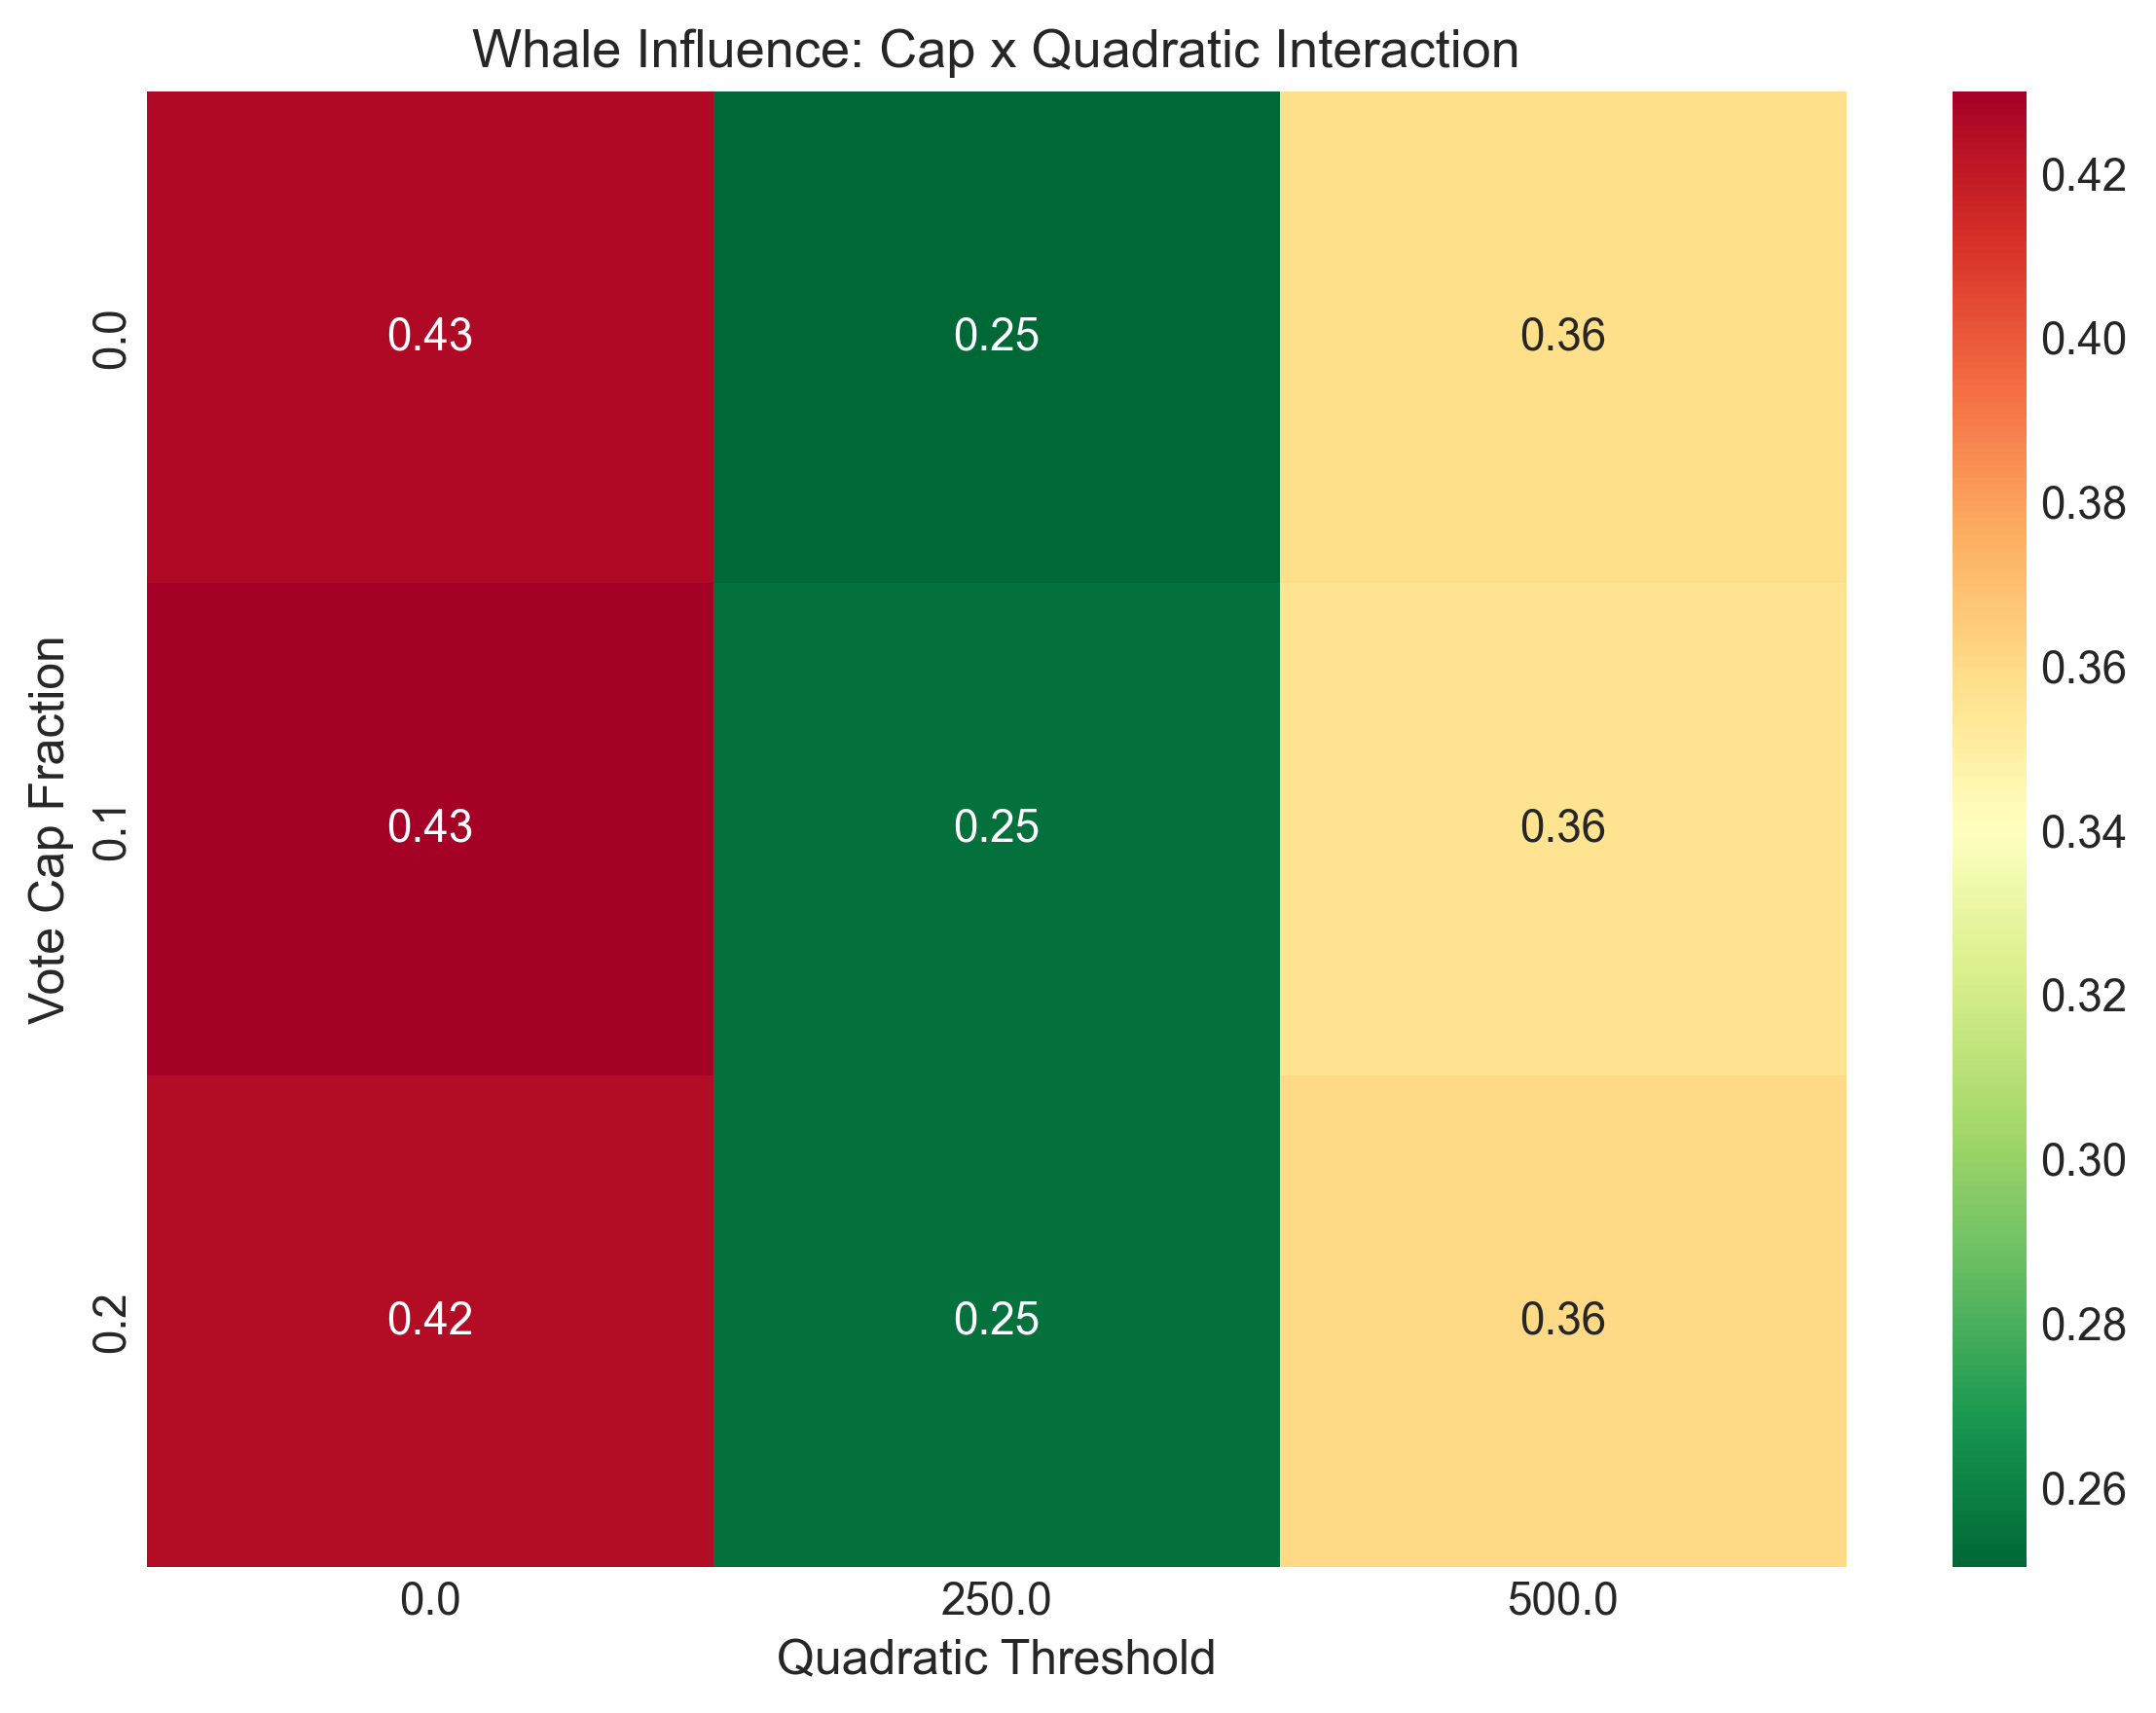
\includegraphics[width=0.8\textwidth]{../figures/rq2_interactions}
    \caption{Heatmap of capture risk across mechanism combinations. Darker colors indicate lower capture risk (better). Combined mechanisms show synergistic effects.}
    \label{fig:rq2-interactions}
\end{figure}

\begin{table}[htbp]
\centering
\caption{Top configurations by capture resistance}
\label{tab:rq2-top-configs}
\begin{tabular}{llllcc}
\toprule
Rank & Cap & Quadratic & Velocity & Capture Risk & Pass Rate \\
\midrule
\pl{1} & \pl{--} & \pl{--} & \pl{--} & \pl{--} & \pl{--} \\
\pl{2} & \pl{--} & \pl{--} & \pl{--} & \pl{--} & \pl{--} \\
\pl{3} & \pl{--} & \pl{--} & \pl{--} & \pl{--} & \pl{--} \\
\bottomrule
\end{tabular}
\end{table}

\subsection{Capture vs. Throughput Tradeoff}

\begin{figure}[htbp]
    \centering
    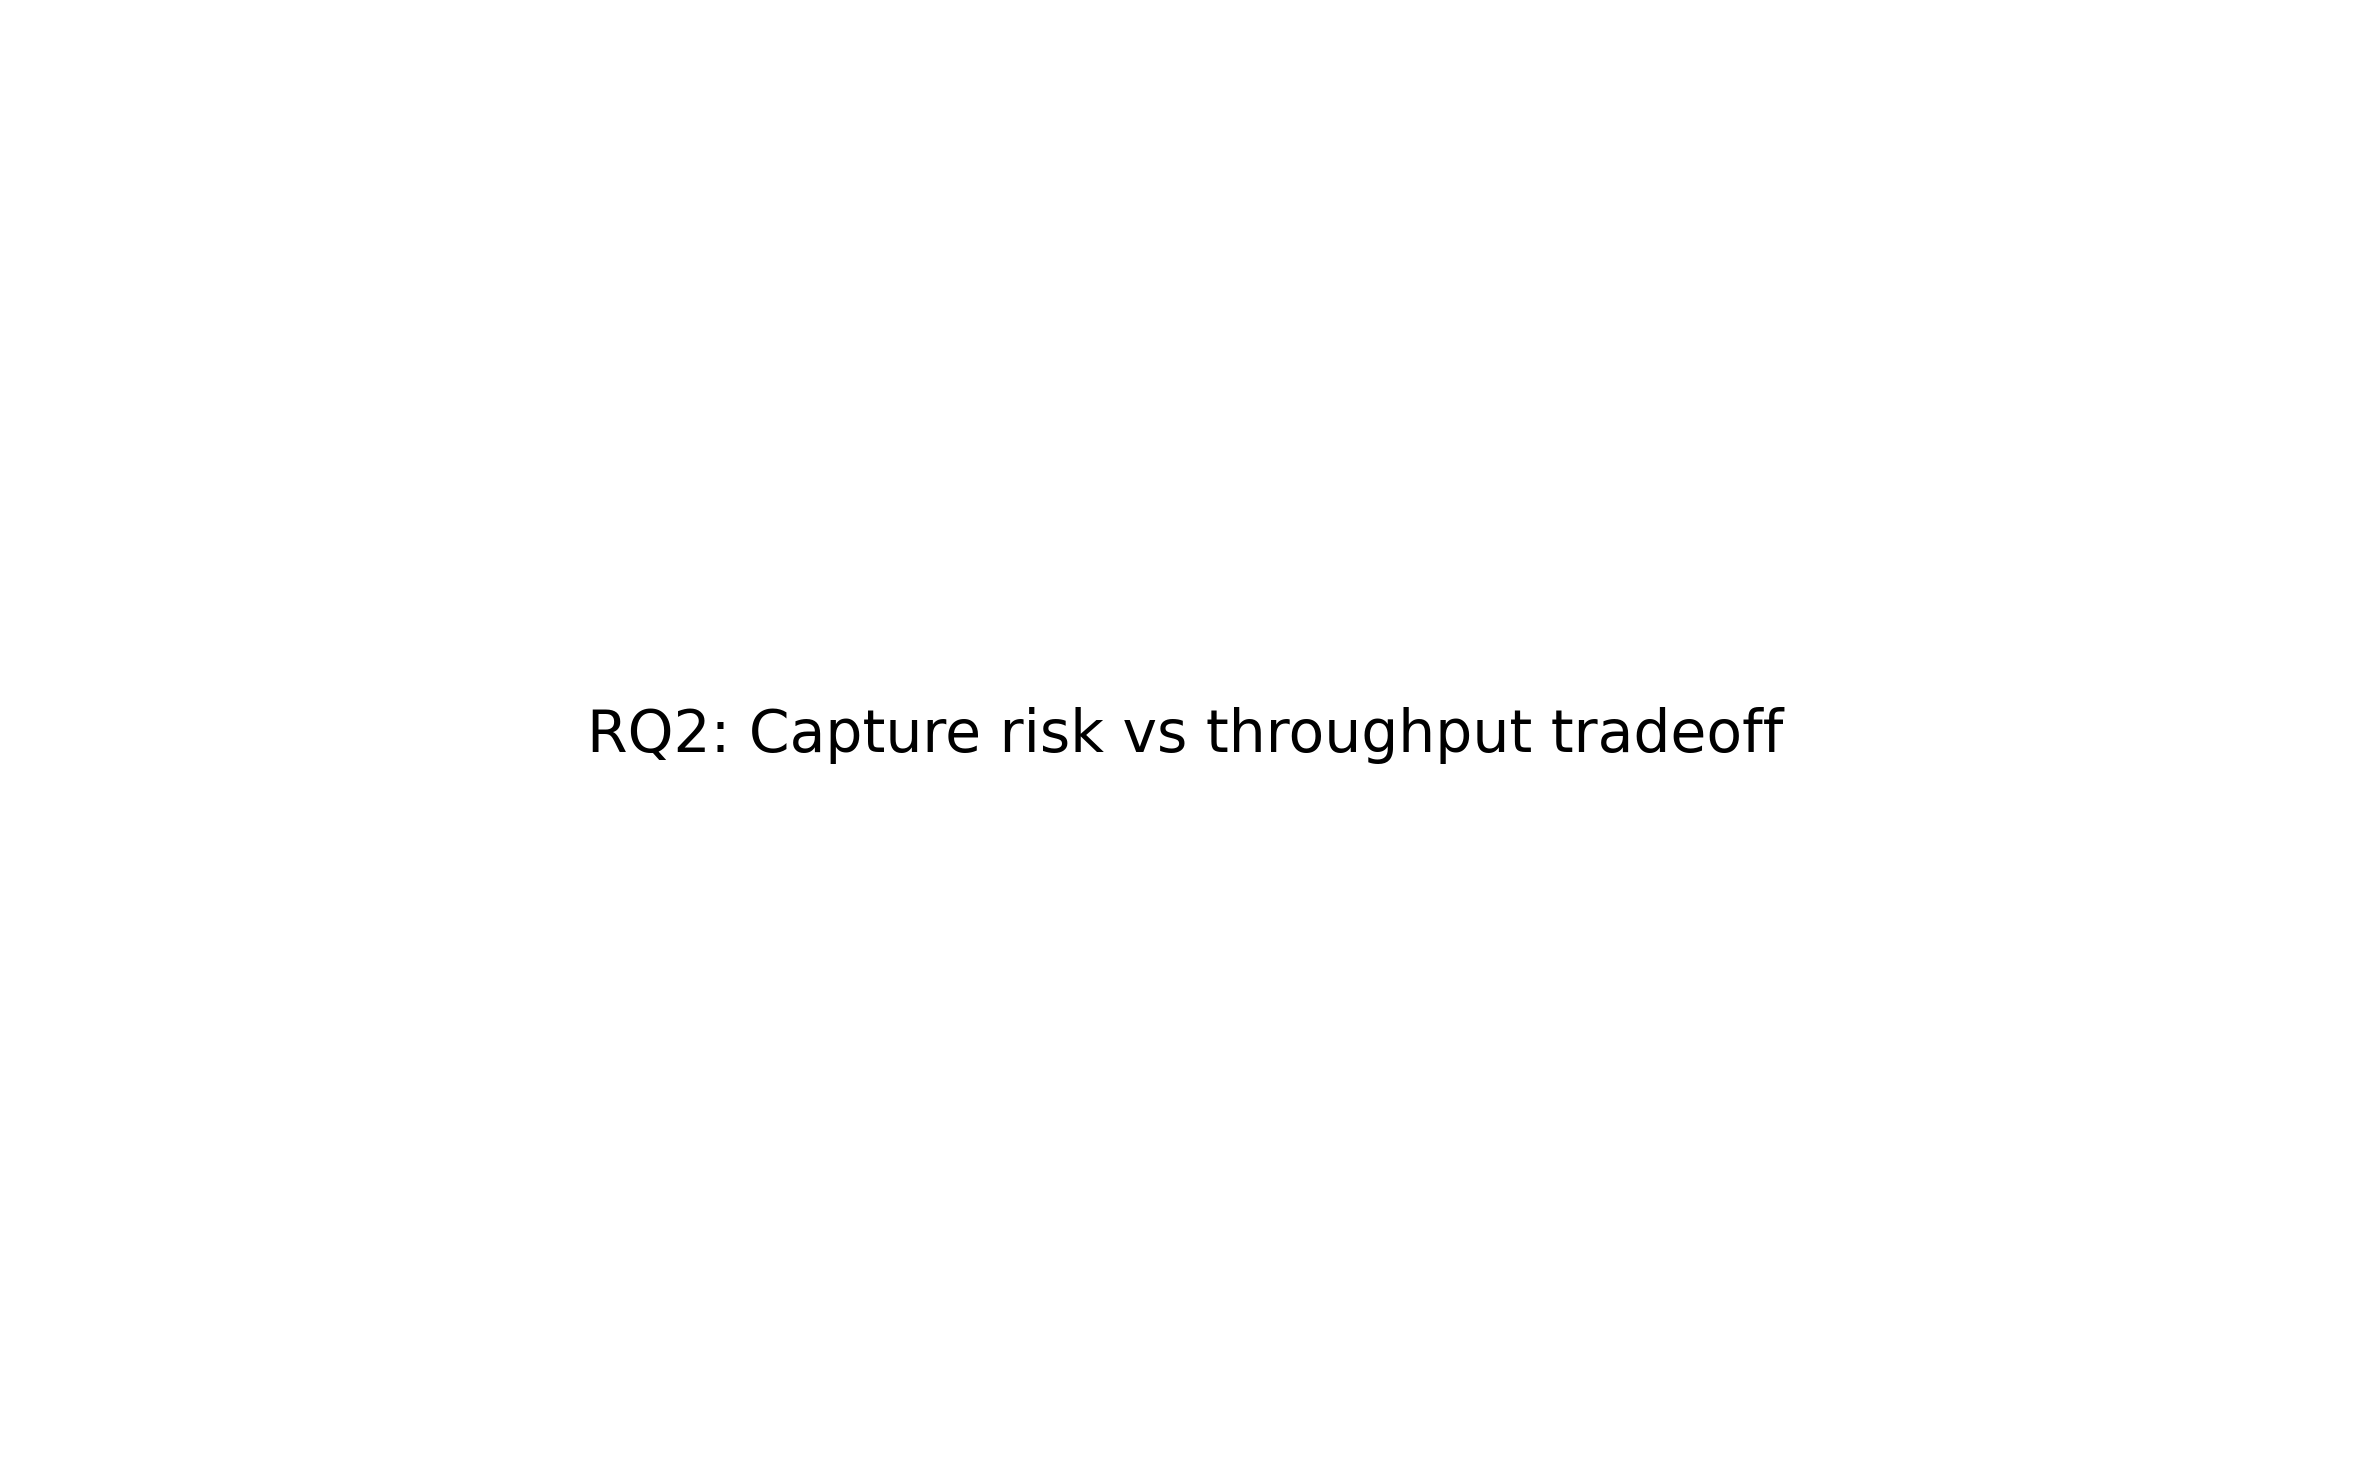
\includegraphics[width=0.8\textwidth]{../figures/rq2_tradeoff}
    \caption{Pareto frontier of capture resistance vs. governance throughput. Points on the frontier represent optimal configurations---improving one metric necessarily harms the other.}
    \label{fig:rq2-tradeoff}
\end{figure}

\subsection{Hypothesis Evaluation}

\begin{table}[htbp]
\centering
\caption{Hypothesis testing results}
\label{tab:rq2-hypotheses}
\begin{tabular}{llcc}
\toprule
Hypothesis & Test & $p$-value & Result \\
\midrule
H2.1: Caps reduce whale influence & ANOVA & \pl{--} & \pl{TBD} \\
H2.2: Quadratic compresses Gini $\sim$50\% & t-test & \pl{--} & \pl{TBD} \\
H2.3: Velocity prevents attacks & Attack simulation & \pl{--} & \pl{TBD} \\
H2.4: Combined $>$ single mechanism & Interaction term & \pl{--} & \pl{TBD} \\
H2.5: Aggressive mitigation $\downarrow$ pass rate & Regression & \pl{--} & \pl{TBD} \\
\bottomrule
\end{tabular}
\end{table}

\subsection{Key Findings}

\begin{enumerate}
    \item \textbf{Vote caps effective but blunt}: 2\% caps reduce whale influence substantially but create cliff effects and sybil incentives

    \item \textbf{Quadratic provides smooth compression}: Square root scaling roughly halves Gini coefficient without hard cutoffs

    \item \textbf{Velocity complements other mechanisms}: Prevents rapid accumulation attacks; most valuable in combination

    \item \textbf{No free lunch}: All mitigation mechanisms impose some governance efficiency cost; optimal choice depends on priorities

    \item \textbf{Hybrid approaches dominate}: Best capture resistance comes from combining mechanisms (e.g., moderate cap + quadratic)
\end{enumerate}
